\chapter{Mitigation Strategies}


\section{Nature-based Solutions}

When it comes to Nature-based solutions, the question arises what this definition means. A quite general definition of nature based solutions would be;

\textit{“Nature-based Solutions are actions to protect, conserve, restore, sustainably
use and manage natural or modified terrestrial, freshwater, coastal and marine
ecosystems, which address social, economic and environmental challenges
effectively and adaptively, while simultaneously providing human well-being,
ecosystem services, resilience and biodiversity benefits” (United Nations, 2022,
p. 2)}

Although this definition may give a thought that it only concerns natural and biodiversity increasing ideas this is actually not the case. For example the impact of NBS on the local economies and communities is of an equal importance. When it comes to weighing the different NBS against each other this report will make use of the seven goals of the IUCN which must be achieved as good as possible. The seven goals are presented below;

\begin{figure}[H]
    \centering
    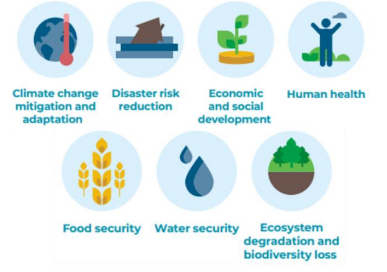
\includegraphics[width=0.50\linewidth]{figures/ThesevenNBSgoals.png}
    \caption{Seven goals for achieving a good NBS}
    \label{fig:placeholder}
\end{figure}

\subsection{Resistance against NBS}

Although NBS are widely known in the scientific world, most people have never heard of these solutions. So, when implementing a solution which can't be described as a classical solution, there is a big change of getting resistance from multiple stakeholders. Especially local communities are skeptical because the solution is less concrete than a classical solution would be. The business case of a NBS must of course also be solid. Without funding of the project, there will never be a change to realize it. That's why it's from great importance to have a solution which is both profitable as explainable to the stakeholders. 

\subsection{Implementing NBS in this project}

As stressed out before in this report, is there a problem with riverbank erosion due to activities on the river. To mitigate or even solve this problem, it is our intend to use a nature based solution. Therefore there are presented multiple possible solutions to create a long-lasting, sustainable riverbank which is made cost effective. These solutions are all graded from one to ten for the seven goals described in section 7.1. The solution which has the highest score will be chosen to mitigate the bank erosion.

One of these solutions is to make a, so said, buffer zone. This means that there is made a swamp area of about 2-8 meter. This gives a change for plants which will hold the soil together. By holding the soil together there will in time be a muddy and organic soil composition, which gives a lot of room for plants and animals to flourish. By doing so, there won't be any erosion on the banks of the river. 


\section{Bed and bank protection measures}

belangrijke/interessante info over deltas en wetlands:
The Paraná Delta, the end of the Paraná-Paraguay river wetland system, begins in the city of Diamante in Entre Ríos province. It stretches for 300 kilometres and covers some 2.3 million hectares. Dotted with islands, these wetlands are a source of ecosystem services such as flood and drought buffering, water purification, erosion control and coastal protection, climate regulation, as well as the provision of shelter, feeding and breeding sites for various wildlife species. It also provides resources including fish, foraging, timber, medicine, and materials for construction and clothing.

In recent years, wetlands have become increasingly important for another key reason: their role as allies against climate change. They improve the resilience of communities to its impacts, serve as natural barriers against floods and droughts, and also function as carbon sinks. Despite playing these important roles, these ecosystems remain under great threat from human action – it is estimated that globally, 85 percent of the wetlands that existed three centuries ago have been destroyed or drastically transformed. 

https://dialogue.earth/en/climate/on-the-parana-river-ecological-crisis-is-a-threat-to-its-identity/


\newpage

\section{Structural Solutions}
There are a number of retaining structures that can be used to stabilize the river banks. Possibilities include:
\begin{itemize}
    \item Sheet pile wall\
    Sheet pile walls are a common retaining structure and consist of vertical barriers made of interlocking sections. They are a lightweight option and can be removed, which makes them reusable across multiple projects. Another advantage is the fact that installation is relatively easy and therefore cheap. However, sheet pile walls also have limitations. In hard soils and soils with boulders or cobbles, installation becomes difficult. Further, installation can disturb nearby areas through sounds and vibrations. These vibrations can even cause settlements to occur.

    \item Diaphragm wall\
    Diaphragm walls are deep, reinforced concrete retaining structures. They provide excellent structural stability and are capable of resisting significant lateral soil and water pressures. One of their key advantages is water tightness, as they effectively prevent groundwater seepage. They are also suitable for a wide range of soil conditions, and offer durability due to the use of reinforced concrete. On the downside, they are costly to build and require significant time and space due to the specialized equipment, skilled labor, and extensive excavation work that is needed.
    
    \item Precast concrete\
    Precast concrete walls are constructed by manufacturing structural elements in a factory environment before transporting them to the construction site. This process allows for superior quality control. Moreover, precast construction can significantly speed up project timelines, as elements are produced in large quantities and quickly installed on-site. Precast concrete offers a long service life with minimal maintenance. Drawbacks of precast concrete walls include: the elements are heavy and thus require specialized transportation and installation equipment. Further, the production and transport processes have notable environmental impacts, and repairs or replacements can be complex and costly.

    \item Auger pile wall or soldier pile wall
    Auger pile walls and soldier pile walls are widely used in construction for retaining slopes. Auger pile walls are formed by drilling and casting concrete in place, while soldier pile walls consist of vertical steel or timber H-piles with horizontal boards or panels placed between them. They are generally cost-effective solutions that generate minimal vibrations, making them suitable for urban areas and sites sensitive to noise or disturbance. Both systems offer flexibility, allowing adjustments to pile placement, size, and depth to suit specific project requirements. However, leakage between adjacent piles is a relevant risk when it comes to these types of walls. Maintaining proper overlap between piles is also critical to ensure structural stability and continuity of the wall.

    \item Embankment
\end{itemize}



Background bespreken en laten zien verschillende opties die mogelijk zijn. Retaining wall en sheet piles. Conclusie in dit rapport zal verder gekeken worden naar een desgin van sheet piles.

\subsection{Sheet Piles}

Hier bespreken wat sheet piles zijn en in welke situaties we deze kunnen gebruiken. Wellicht een case study bespreken van Pampana waar in een delta achtige rivier dezelfde methode is weten toe te passen.

\subsubsection{Materials}

Hier bespreken van welke materialen deze sheet piles zijn gemaakt in practice.

\subsubsection{Case Study}

Bekijken in de literatuur naar voorbeelden van deze manier van sheet piles in rivieren.

\subsubsection{Cantilever Sheet Piling}

Hier bespreken en laten zien wat cantilever sheet piling is. 

\subsubsection{Failure Mechanisms}

Bespreken wat de mogelijke faal mechanismen zijn van het gerbuik van sheet piles.

\subsubsection{Structural Requirements}

\subsection{Design Methods}

Hier bespreken welke desgin methode we gaan gebruiken. Active en Passive kant van de sheet pile bepalen. Kracht horizontal en momenten som aan nul gelijk stellen om daarmee te bepalen wat de D van de sheet pile moet zijn. Hier een factor overheen gooien. 

\subsection{Design Procedure}

Hier komt de procedure te staan hoe het design tot stand zal gaan komen en welke stappen gemaakt zullen worden.

\subsubsection{Problem Description}

Hier komt een schets van de situatie.

\subsubsection{Geometry of Design}

Hier komt te staan wat de lengte en diepte van de sheet piles zullen worden. En welk profiel gebruikt zal worden voor de sheet piles.

\subsubsection{Internal Loads}

\subsection{Conclusion}

